\documentclass{article}
\usepackage[utf8]{inputenc}
\usepackage{csquotes}
\usepackage{natbib}
\usepackage{graphicx}
\usepackage{float} 
\usepackage{epsfig}
\usepackage{siunitx}
\begin{document}
\begin{titlepage}
	\begin{center}
		\Huge\textbf{EE-568 }\\
		\vspace{0.5cm}
		\Huge\textbf{HW-2}\\
		\vspace{0.5cm}
		\Huge\textbf{Motor Winding Design and Analysis}\\
		\vspace{0.5cm}
		
\includegraphics[scale=1]{E:/Github/EE568/HW1/Rapor/Figurler/odtulogo}\\
		
		
		\Large\textbf{Prepared by:}Hakan POLAT\\
		
		\Large\textbf{Submitted to:} Dr. Ozan KEYSAN\\
		\vspace{0.5cm}
		\Large\textbf{Electrical and Electronics Engineering Department}\\
		
		\large\textbf{ANKARA	}\\
		\large\textbf{31.03.2020}\\	
		
		
	\end{center}
	
	

\end{titlepage}
\tableofcontents
\newpage
\section{Introduction}
This report consists of 4 parts. In the first section an analysis on aq 20-pole 120 slot 3-phase permanent magnet machine will be made. In the next section a fractional-slot winding design will be presented where a pole number 20 or 22 will be selected. Then a slot number between 20-30 will be selected usioıng Emetor Winding Design. Then various analysis will be delivered. In the last section, a fractional slot PMSM will be analyzed usign ANSYS Maxwell finite element analysis(FEA) where a general 2D drawing and winding diagram will be presented. Then the airgap flux distribution and the induced voltage waveforms (phase and line-line) at rated speed will be given. Finally the cogging torque of the proposed machine will be investigated.

\section{Integral-Slot Winding Design}
In this section it is assumed that the PMSM has 20-poles, 120-slot and the number of phases is three. As for $\mathrm{\lambda}$
a full pitch design is selected and hence $\mathrm{\lambda=1}$. Then slots per pole por phase ,denoted as q, can be calculated as in Eq. \ref{eq:q_integral} .
\begin{equation}
	q=\frac{120}{20x3}=2
	\label{eq:q_integral}
\end{equation}
Moreover, it is clear that there are in total of 6 slots per pole and hence the winding diagram of a sinle pole-pair is given in Table \ref{tab:winding_integral} .

\begin{table}[H]
	\caption{Winding Diagram of a Single Pole-Pair}
	\label{tab:winding_integral}
	\begin{tabular}{llllllllllll}
	1	& 2 &3  &4  & 5 & 6 & 7 & 8 & 9 &10  &11  &12  \\
	A1	& A2 & -C1 & -C2 & B1 &B2  & -A1 & -A2 &C1  & C2 & -B1 & -B2
	\end{tabular}
\end{table}
Then the distribution factor, pitch factor and the winding factor for the fumdamental component can be calculated as in Eq., Eq. and Eq. respectively.

\begin{equation}
k_d=\frac{sin(q\frac{\alpha}{2})}{qsin(\frac{\alpha}{2})}=0.965
\label{eq:kp_integral}
\end{equation}

\begin{equation}
k_p=sin(\frac{\lambda}{2})=sin(\frac{180}{2})=1
\label{eq:kd_integral}
\end{equation}

\begin{equation}
k_w=k_pxk_d=k_d=0.965
\label{eq:qkw_integral}
\end{equation}

The same procedure can be generalized for the n-th harmonic of the input voltage waveform. However, in three phase machines the 3-rd and 5-th 7-th harmonics are often under investigation since the rest of the harmonic have relatively low magnitudes. In this question the 3-rd and 5-th harmonics are calculated.\\
The $k_p$, $k_d$ and $k_w$ for 3-rd harmonic are given in Eq. \ref{eq:kp3_integral}, Eq.\ref{eq:kd3_integral} and Eq. \ref{eq:qkw3_integral} respectively.

\begin{equation}
k_p=sin(\frac{3\lambda}{2})=sin(\frac{3x180}{2})=-1
\label{eq:kd3_integral}
\end{equation}


\begin{equation}
k_d=\frac{sin(3q\frac{\alpha}{2})}{qsin(\frac{3\alpha}{2})}=0.707
\label{eq:kp3_integral}
\end{equation}

\begin{equation}
k_w=k_pxk_d=k_d=-0.707
\label{eq:qkw3_integral}
\end{equation}

Similarly the $k_p$, $k_d$ and $k_w$ for 5-th harmonic are given in Eq. \ref{eq:kp5_integral}, Eq.\ref{eq:kd5_integral}  and Eq.\ref{eq:qkw5_integral} respectively.

\begin{equation}
k_p=sin(\frac{5\lambda}{2})=sin(\frac{3x180}{2})=1
\label{eq:kd5_integral}
\end{equation}


\begin{equation}
k_d=\frac{sin(5q\frac{\alpha}{2})}{qsin(\frac{5\alpha}{2})}=-0.44
\label{eq:kp5_integral}
\end{equation}

\begin{equation}
k_w=k_pxk_d=k_d= -0.44
\label{eq:qkw5_integral}
\end{equation}


Compared to the fumdamental component 3-rd and 5-th harmonics have high magnitude. This is due to selection of full-pitch winding. If a 144 degrees of coil pitch angle were to be selected, the $k_p=0$ meaning there are no 5-th harmonic flowing in the system. Although the magnitude of the 5-th harmoic is significantly lower than 3-rd harmic pitch-factor is usually selected to reduce the 5-th harmonic. This is due to elimination the 3-rd harmonic when the three phases are connected as a Wye connection.


\section{Fractional-Slot Winding Design}

In this part it is asked to choose a pole number 20 or 22. As for the number of slot any slot number between 20 to 30 can be selected. In order to achieve high winding factor a pole number of 22 was selected. As for the number of slots 24 is selected. During the selection Emetor Winding Design was used.

Firstly the phase angle of the induced voltage in each slot is presented in Table \ref{tab:voltageangle22-24}. 

\begin{table}[H]
	\caption{Angle of Induced Voltage in each Slot}
	\label{tab:voltageangle22-24}
	\begin{tabular}{llllllllllll}
	1	&  2& 3 &4  & 5 & 6 & 7 & 8 & 9 & 10 & 11 & 12 \\
	\hline
	0& 165 &330 &135 &300 &105& 270 &75 &240 &45& 210& 15 \\
		\hline
	13	& 14 & 15 &16  &17  &18  &19  &20  &21  &22  &23  &24  \\
		\hline
	180 &345 &150 &315& 120 &285& 90& 255 &60 &225 &30 &195
	\end{tabular}
\end{table}

In Fig. \ref{fig:22p24svoltage} the vectors for phase-a are present. There is 15 degrees between each voltage vector and hence slots 1, 2, 12, 13, 14, 23, 24 can be used.

\begin{figure}[H]
	\centering
	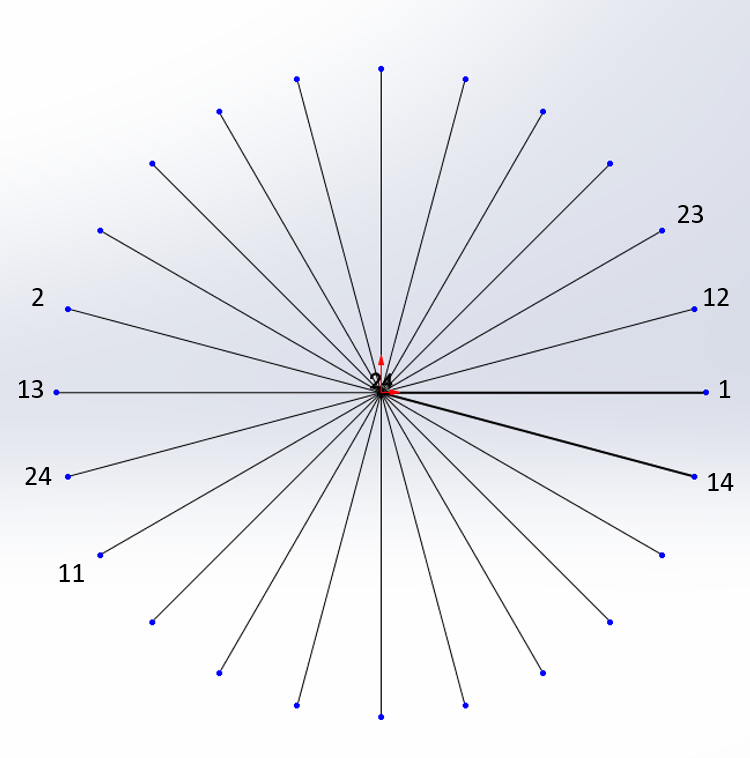
\includegraphics[width=0.7\linewidth]{Figurler/22p24s_voltage}
	\caption{Voltage vector in the selected fractional-slot winding.}
	\label{fig:22p24svoltage}
\end{figure}

Distribution factor can be calculated as the vectoral sum of voltage vectors 23, 12, 1 and 14. Then the $k_d$ can be calculated as in Eq. \ref{eq:kd2022}
\begin{equation}
k_d=\frac{3.82}{4}=0.956
\label{eq:kd2022}
\end{equation}
The pitch factor can be calculated as in Eq. \ref{eq:kp2022}.

\begin{equation}
k_p=sin(165/2)=0.991
\label{eq:kp2022}
\end{equation}
The winding factor can be calculated as Eq. \ref{eq:kw2022}.

\begin{equation}
k_w=k_pxk_d= 0.991x0.956=0.947
\label{eq:kw2022}
\end{equation}

The third and the fifth harmonic can be also be calculated.\\

\begin{equation}
k_p=sin(3*165/2)= 0.924
\label{eq:kp32022}
\end{equation}

\begin{equation}
k_p=sin(5*165/2)= 0.793
\label{eq:kp52022}
\end{equation}

\begin{equation}
k_d=\frac{sin(3x0.36x82.5)}{0.36sin(3x82.5)}=
\label{eq:kd32022}
\end{equation}

\begin{equation}
k_d=\frac{sin(3x0.36x82.5)}{0.36sin(3x82.5)}=
\label{eq:kd52022}
\end{equation}


Then another fractional slot design is made for 20 pole. As for slot number 24 is selected. The electrical angle between two neighbour slots is given in Eq. \ref{eq:188}.

\begin{equation}
Angle=\frac{360}{24}\frac{20}{2}=150
\label{eq:188}
\end{equation}

\begin{table}[H]
	\caption{Angle of Induced Voltage in each Slot}
	\label{tab:voltageangle20-24}
	\begin{tabular}{llllllllllll}
		1	&  2& 3 &4  & 5 & 6 & 7 & 8 & 9 & 10 & 11 & 12 \\
		\hline
		
		0&	150	&300&	90	&240&	30&	180&	330&	120&	270&	60&	210	\\
		\hline
		13	& 14 & 15 &16  &17  &18  &19  &20  &21  &22  &23  &24 \\
			\hline
		0&	150	&300&	90	&240&	30	&180&	330	&120&	270	&60	&210 
	
	\end{tabular}
\end{table}
The voltage angle between each slot is given in Table \ref{tab:voltageangle20-24}.

The voltage vectors are given in Fig. \ref{fig:voltagefrac}.
\begin{figure}[H]
	\centering
	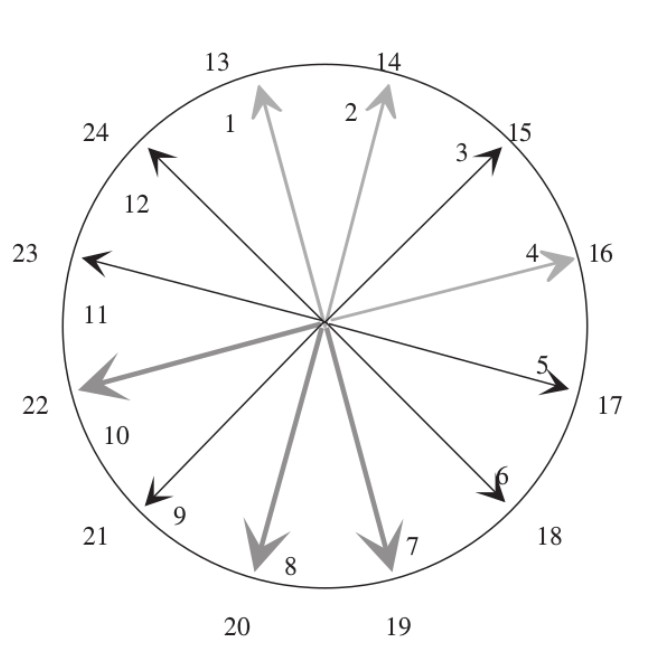
\includegraphics[width=0.7\linewidth]{Figurler/20p24s}
	\caption{Voltage vector in the selected fractional-slot winding.}
	\label{fig:voltagefrac}
\end{figure}

For a single phase slots 1, 13, 8 and 20 forms the A phase. Hence the distribution factor can be calculated as in Eq. \ref{eq:kdfalan}.

\begin{equation}
	k_d=\frac{2*2cos(15)}{4}=0.965
	\label{eq:kdfalan}
\end{equation}
 If A+ is wound on slot number 1, A- can be connected to slot 2. Hence the pitch factor is given in Eq.\ref{eq:kpfalan}
 
 \begin{equation}
 k_p=sin(150/2)=0.965
 \label{eq:kpfalan}
 \end{equation}
  Which results in a winding factor given in Eq. \ref{eq:kwfalan}
  
   \begin{equation}
  k_w=kpxkd=0.965*0.965=0.933
  \label{eq:kwfalan}
  \end{equation}
  
 For the third harmonic the winding factor can be calculated as in Eq.\ref{eq:kw3falan}. 
 
    \begin{equation}
  k_w=kpxkd=\frac{sin(3q\alpha/2)}{qsin(3\alpha/2)}sin(3\lambda/2)=0.707x -0.707=-0.5
  \label{eq:kw3falan}
  \end{equation}
  For the fifth harmonic the winding factor can be calculated as in Eq. \ref{eq:kw5falan}.
  
  \begin{equation}
  k_w=kpxkd=\frac{sin(5q\alpha/2)}{qsin(5\alpha/2)}sin(3\lambda/2)=-0.707x 0.258=0.183 
  \label{eq:kw5falan}
  \end{equation}
  
  
  I couldnt do the necessary calculations for the 22pole 24 slot case. 
  
 \section{2D FEA of 20 Pole 24 Slot PMSM}
 
 The geometry of a 20 pole 224 slot machine is given in Fig. \ref{fig:feageom}.
 

\begin{figure}[H]
	\centering
	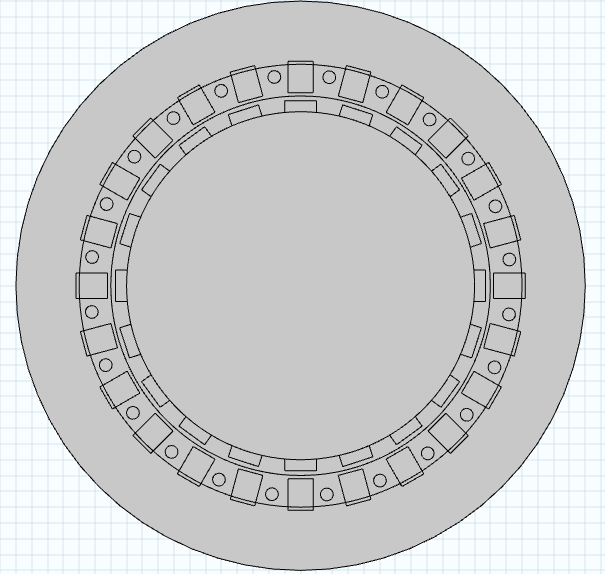
\includegraphics[width=0.7\linewidth]{Figurler/FEAgeom}
	\caption{Motor Geometry}
	\label{fig:feageom}
\end{figure}

During operation the magnetic field is given in Fig. \ref{fig:magneticfield}

\begin{figure}[H]
	\centering
	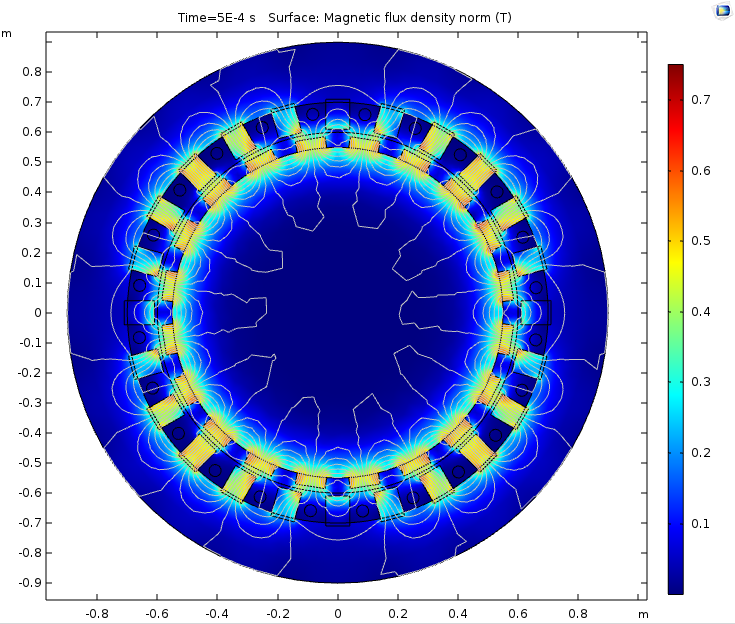
\includegraphics[width=0.7\linewidth]{Figurler/magneticfield}
	\caption{Airgap flux density distribution}
	\label{fig:magneticfield}
\end{figure}
 The induced voltages are given in Fig. \ref{fig:phasevoltages}
 
\begin{figure}[H]
	\centering
	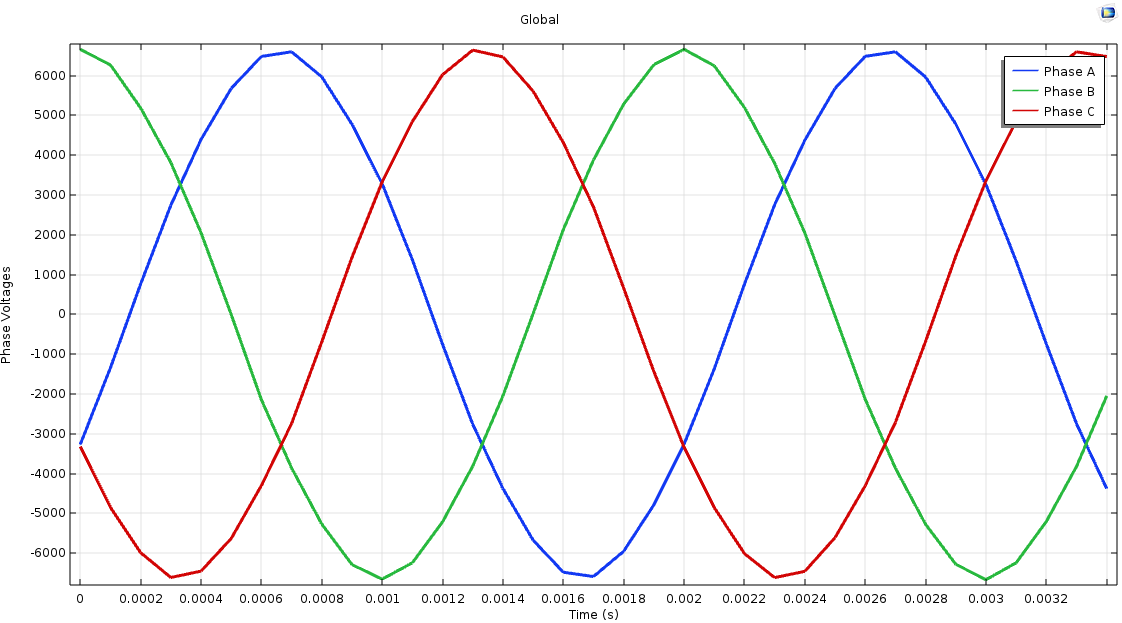
\includegraphics[width=0.7\linewidth]{Figurler/phasevoltages}
	\caption{Induced voltages per phase}
	\label{fig:phasevoltages}
\end{figure}
 
 The cogging torque is given in Fig. \ref{fig:cogging}.
 
\begin{figure}[H]
	\centering
	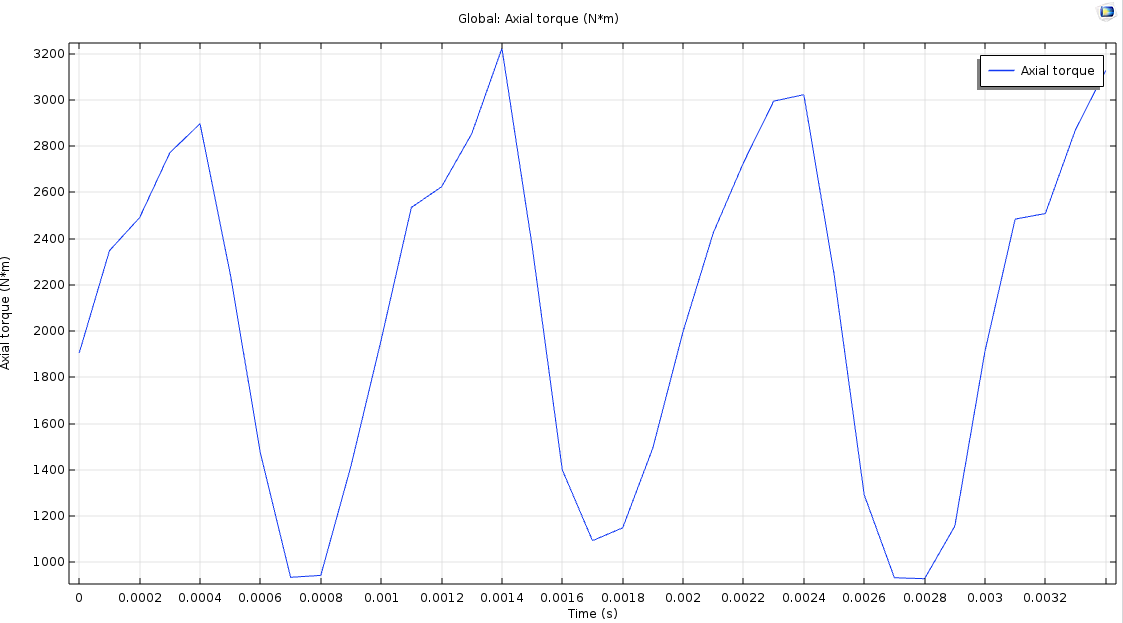
\includegraphics[width=0.7\linewidth]{Figurler/cogging}
	\caption{Cogging Torque}
	\label{fig:cogging}
\end{figure}
Also a 3d moving gif of the motor is in the Github repository. 
 \section{Conclusion}
 In this homework, it was asked to desing various PMSM machine windings where concepts like pitch factor, distribution factor and winding factor was under investigation. The effect of winding design on the harmonic content was also discussed.

\end{document}